\section{Model3DRigid\-Chain  Class Reference}
\label{classModel3DRigidChain}\index{Model3DRigidChain@{Model3DRigid\-Chain}}
A 3D kinematic chain of bodies that uses DH parameters. 


{\tt \#include $<$model3d.h$>$}

Inheritance diagram for Model3DRigid\-Chain::\begin{figure}[H]
\begin{center}
\leavevmode
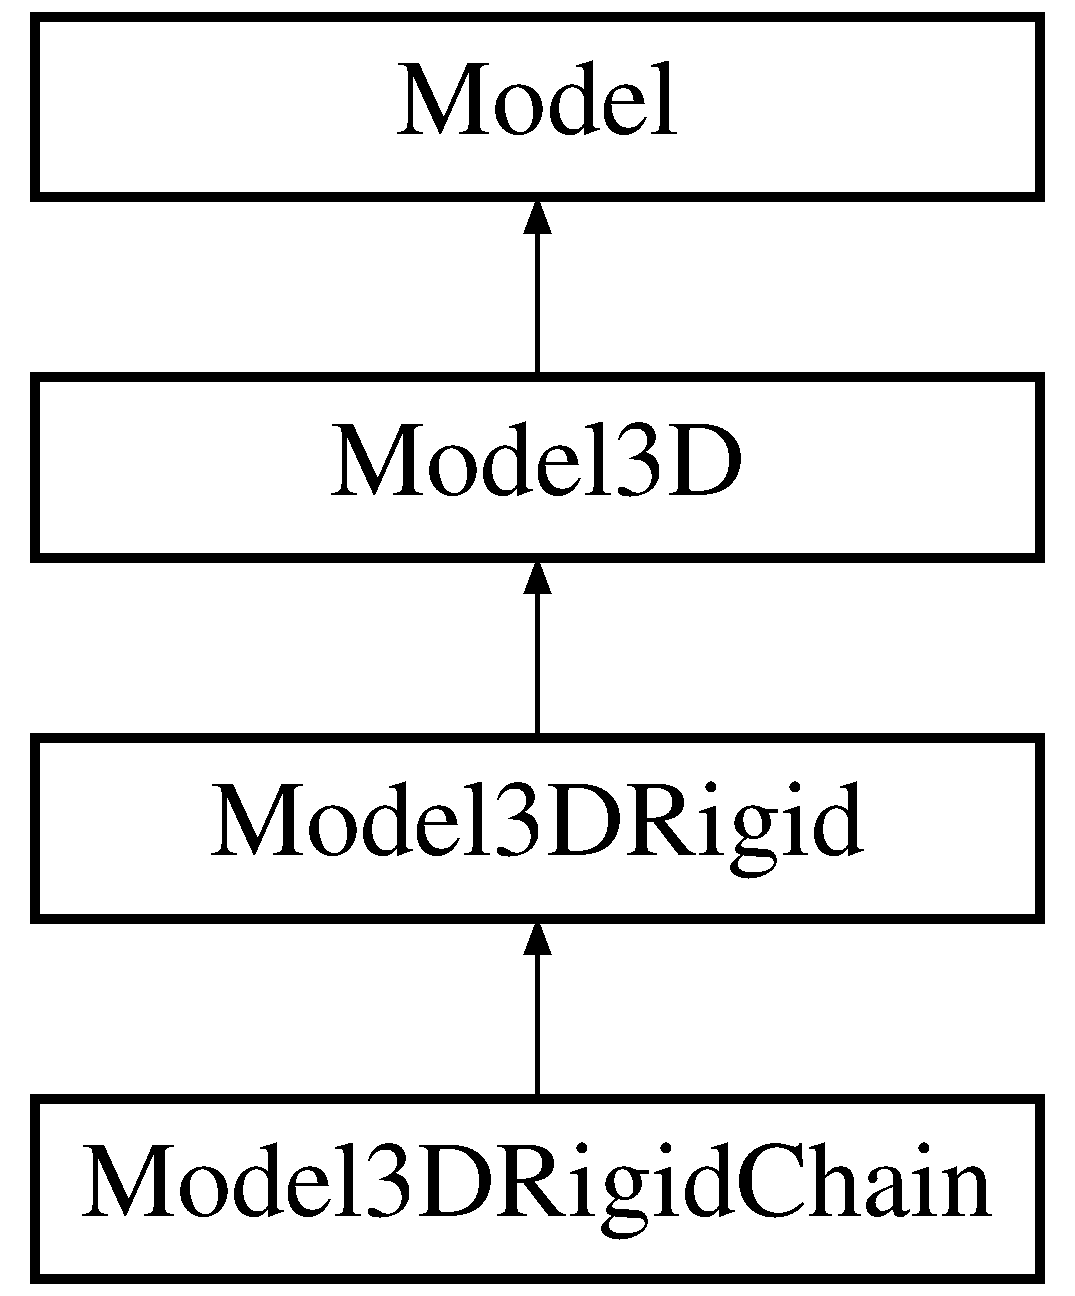
\includegraphics[height=4cm]{classModel3DRigidChain}
\end{center}
\end{figure}
\subsection*{Public Methods}
\begin{CompactItemize}
\item 
{\bf Model3DRigid\-Chain} (string path)
\item 
virtual {\bf $\sim$Model3DRigid\-Chain} ()
\item 
virtual {\bf MSLVector} {\bf State\-Transition\-Equation} (const {\bf MSLVector} \&{\bf x}, const {\bf MSLVector} \&u)
\begin{CompactList}\small\item\em The state transition equation, or equations of motion, xdot=f(x,u).\item\end{CompactList}\item 
virtual {\bf MSLVector} {\bf State\-To\-Configuration} (const {\bf MSLVector} \&{\bf x})
\begin{CompactList}\small\item\em A method that converts a {\bf Model} {\rm (p.\,\pageref{classModel})} state in to a {\bf Geom} {\rm (p.\,\pageref{classGeom})} configuration.\item\end{CompactList}\item 
virtual double {\bf Metric} (const {\bf MSLVector} \&x1, const {\bf MSLVector} \&x2)
\begin{CompactList}\small\item\em A distance metric, which is Euclidean in the base class.\item\end{CompactList}\item 
virtual bool {\bf Satisfied} (const {\bf MSLVector} \&{\bf x})
\begin{CompactList}\small\item\em Test whether global state-space constraints are satisfied.\item\end{CompactList}\end{CompactItemize}
\subsection*{Public Attributes}
\begin{CompactItemize}
\item 
int {\bf Num\-Bodies}
\begin{CompactList}\small\item\em Number of bodies in the chain.\item\end{CompactList}\item 
{\bf MSLVector} {\bf DH}
\begin{CompactList}\small\item\em The distances between joints (\char`\"{}a\char`\"{} parameters in kinematics).\item\end{CompactList}\item 
vector$<$ int $>$ {\bf State\-Indices}
\end{CompactItemize}


\subsection{Detailed Description}
A 3D kinematic chain of bodies that uses DH parameters.

A 3D kinematic chain of bodies that uses DH parameters that should be given in a DH file in the following order: Alpha(1,2...), Theta(1,2...), A(1,2...), D(1,2...). Some of these parameters change during the movement, and each of these parameters becomes a state variable. The indices of these parameters should be given in the file State\-Indices (i.e., each entry corresponds to a state, and indicates which DH parameter is variable). 



\subsection{Constructor \& Destructor Documentation}
\index{Model3DRigidChain@{Model3DRigid\-Chain}!Model3DRigidChain@{Model3DRigidChain}}
\index{Model3DRigidChain@{Model3DRigidChain}!Model3DRigidChain@{Model3DRigid\-Chain}}
\subsubsection{\setlength{\rightskip}{0pt plus 5cm}Model3DRigid\-Chain::Model3DRigid\-Chain (string {\em path})}\label{classModel3DRigidChain_a0}


\index{Model3DRigidChain@{Model3DRigid\-Chain}!~Model3DRigidChain@{$\sim$Model3DRigidChain}}
\index{~Model3DRigidChain@{$\sim$Model3DRigidChain}!Model3DRigidChain@{Model3DRigid\-Chain}}
\subsubsection{\setlength{\rightskip}{0pt plus 5cm}virtual Model3DRigid\-Chain::$\sim$Model3DRigid\-Chain ()\hspace{0.3cm}{\tt  [inline, virtual]}}\label{classModel3DRigidChain_a1}




\subsection{Member Function Documentation}
\index{Model3DRigidChain@{Model3DRigid\-Chain}!Metric@{Metric}}
\index{Metric@{Metric}!Model3DRigidChain@{Model3DRigid\-Chain}}
\subsubsection{\setlength{\rightskip}{0pt plus 5cm}double Model3DRigid\-Chain::Metric (const {\bf MSLVector} \& {\em x1}, const {\bf MSLVector} \& {\em x2})\hspace{0.3cm}{\tt  [virtual]}}\label{classModel3DRigidChain_a4}


A distance metric, which is Euclidean in the base class.



Reimplemented from {\bf Model3DRigid} {\rm (p.\,\pageref{classModel3DRigid_a4})}.\index{Model3DRigidChain@{Model3DRigid\-Chain}!Satisfied@{Satisfied}}
\index{Satisfied@{Satisfied}!Model3DRigidChain@{Model3DRigid\-Chain}}
\subsubsection{\setlength{\rightskip}{0pt plus 5cm}bool Model3DRigid\-Chain::Satisfied (const {\bf MSLVector} \& {\em x})\hspace{0.3cm}{\tt  [virtual]}}\label{classModel3DRigidChain_a5}


Test whether global state-space constraints are satisfied.



Reimplemented from {\bf Model} {\rm (p.\,\pageref{classModel_a4})}.\index{Model3DRigidChain@{Model3DRigid\-Chain}!StateToConfiguration@{StateToConfiguration}}
\index{StateToConfiguration@{StateToConfiguration}!Model3DRigidChain@{Model3DRigid\-Chain}}
\subsubsection{\setlength{\rightskip}{0pt plus 5cm}{\bf MSLVector} Model3DRigid\-Chain::State\-To\-Configuration (const {\bf MSLVector} \& {\em x})\hspace{0.3cm}{\tt  [virtual]}}\label{classModel3DRigidChain_a3}


A method that converts a {\bf Model} {\rm (p.\,\pageref{classModel})} state in to a {\bf Geom} {\rm (p.\,\pageref{classGeom})} configuration.



Reimplemented from {\bf Model} {\rm (p.\,\pageref{classModel_a8})}.\index{Model3DRigidChain@{Model3DRigid\-Chain}!StateTransitionEquation@{StateTransitionEquation}}
\index{StateTransitionEquation@{StateTransitionEquation}!Model3DRigidChain@{Model3DRigid\-Chain}}
\subsubsection{\setlength{\rightskip}{0pt plus 5cm}{\bf MSLVector} Model3DRigid\-Chain::State\-Transition\-Equation (const {\bf MSLVector} \& {\em x}, const {\bf MSLVector} \& {\em u})\hspace{0.3cm}{\tt  [virtual]}}\label{classModel3DRigidChain_a2}


The state transition equation, or equations of motion, xdot=f(x,u).



Reimplemented from {\bf Model3DRigid} {\rm (p.\,\pageref{classModel3DRigid_a3})}.

\subsection{Member Data Documentation}
\index{Model3DRigidChain@{Model3DRigid\-Chain}!DH@{DH}}
\index{DH@{DH}!Model3DRigidChain@{Model3DRigid\-Chain}}
\subsubsection{\setlength{\rightskip}{0pt plus 5cm}{\bf MSLVector} Model3DRigid\-Chain::DH}\label{classModel3DRigidChain_m1}


The distances between joints (\char`\"{}a\char`\"{} parameters in kinematics).

\index{Model3DRigidChain@{Model3DRigid\-Chain}!NumBodies@{NumBodies}}
\index{NumBodies@{NumBodies}!Model3DRigidChain@{Model3DRigid\-Chain}}
\subsubsection{\setlength{\rightskip}{0pt plus 5cm}int Model3DRigid\-Chain::Num\-Bodies}\label{classModel3DRigidChain_m0}


Number of bodies in the chain.

\index{Model3DRigidChain@{Model3DRigid\-Chain}!StateIndices@{StateIndices}}
\index{StateIndices@{StateIndices}!Model3DRigidChain@{Model3DRigid\-Chain}}
\subsubsection{\setlength{\rightskip}{0pt plus 5cm}vector$<$int$>$ Model3DRigid\-Chain::State\-Indices}\label{classModel3DRigidChain_m2}




The documentation for this class was generated from the following files:\begin{CompactItemize}
\item 
{\bf model3d.h}\item 
{\bf model3d.C}\end{CompactItemize}
